\documentclass{article}


\usepackage{arxiv}

\usepackage[utf8]{inputenc} % allow utf-8 input
\usepackage[T1]{fontenc}    % use 8-bit T1 fonts
\usepackage{hyperref}       % hyperlinks
\usepackage{url}            % simple URL typesetting
\usepackage{booktabs}       % professional-quality tables
\usepackage{amsfonts}       % blackboard math symbols
\usepackage{nicefrac}       % compact symbols for 1/2, etc.
\usepackage{microtype}      % microtypography
\usepackage{lipsum}


%%%% Start: Added by Sanam 
\usepackage{tcolorbox}
\usepackage{graphicx}
\usepackage{makecell}
\usepackage{float}
%%%% End: Added by Sanam 


\title{Designing the Elements of a 2D Beam Scanner for a High Speed and High Resolution LiDAR}
%\title{A template for the \emph{arxiv} style}



\author{
  Sanam Moslemi Tabriz %\thanks{Use footnote for providing further
%    information about author (webpage, alternative
%    address)---\emph{not} for acknowledging funding agencies.} 
\\
  Department of Electronics\\
  Carleton University\\
%  Pittsburgh, PA 15213 \\
%  \texttt{hippo@cs.cranberry-lemon.edu} \\
%  %% examples of more authors
%   \And
% Elias D.~Striatum \\
%  Department of Electrical Engineering\\
%  Mount-Sheikh University\\
%  Santa Narimana, Levand \\
%  \texttt{stariate@ee.mount-sheikh.edu} \\
%  %% \AND
%  %% Coauthor \\
%  %% Affiliation \\
%  %% Address \\
%  %% \texttt{email} \\
%  %% \And
%  %% Coauthor \\
%  %% Affiliation \\
%  %% Address \\
%  %% \texttt{email} \\
%  %% \And
%  %% Coauthor \\
%  %% Affiliation \\
%  %% Address \\
%  %% \texttt{email} \\
}



%\author{
%  David S.~Hippocampus\thanks{Use footnote for providing further
%    information about author (webpage, alternative
%    address)---\emph{not} for acknowledging funding agencies.} \\
%  Department of Computer Science\\
%  Cranberry-Lemon University\\
%  Pittsburgh, PA 15213 \\
%  \texttt{hippo@cs.cranberry-lemon.edu} \\
%  %% examples of more authors
%   \And
% Elias D.~Striatum \\
%  Department of Electrical Engineering\\
%  Mount-Sheikh University\\
%  Santa Narimana, Levand \\
%  \texttt{stariate@ee.mount-sheikh.edu} \\
%  %% \AND
%  %% Coauthor \\
%  %% Affiliation \\
%  %% Address \\
%  %% \texttt{email} \\
%  %% \And
%  %% Coauthor \\
%  %% Affiliation \\
%  %% Address \\
%  %% \texttt{email} \\
%  %% \And
%  %% Coauthor \\
%  %% Affiliation \\
%  %% Address \\
%  %% \texttt{email} \\
%}

\begin{document}
%\maketitle
%
%\begin{abstract}
%%\lipsum[1]
%Light Detection and Ranging (LIDAR) is a very accurate mapping technology in which light is shined toward an object and the reflected beam is observed to map the object precisely. A key part of LiDAR is beam steering. Conventional LiDAR systems use mechanical and/or thermal effect to do the beam steering which are costly and not efficient. In this research in order  to reduce the cost and size and also increase the resolution, speed and field of view (FOV) we focus on a solid state silicon photonic method. The novelty of this research will be in solid state depletion based optical phased array (OPA) phase shifting and sophisticated nonuniform surface grating in order to achieve a hight speed, high resolution and wide 2D beam steering.
%\end{abstract}
%
%
%% keywords can be removed
%\keywords{LiDAR \and 2D Scanning \and Subwavelength grating  (SWG)}
%%\keywords{First keyword \and Second keyword \and More}
%
%
%\section{Introduction}
%
%LiDAR market varies from autonomous vehicles to agriculture, archaeology, modelling of pollution and many more. With growing application specially in car and aviation industries the development of high speed and high resolution LiDAR device is essential. In general a LiDAR system consists of the following block as shown in figure \ref{lidarsys}
%%\begin{figure}[H]
%\begin{figure}[htb]
%\begin{center}
%\includegraphics[width=12cm, height=8cm]{Figures/lidar_block_diagram}
%\caption{A Typical LiDAR System}
%\label{lidarsys}
%\end{center}
%\end{figure}
%
%
%\begin{description}
%\item[Light source:] A tunable laser which can be either be off chip or integrated into the PIC. The source may be modulated and/or pulsed to allow for noise reduction and the detection of object distances and velocities.  
%\item[Splitter:] Various elements can be used to split the source into physically separated  optical channels. For a moderate number of channels, a series of splitters can be used, however, if a larger number of channels is desired a device such as star coupler may be used. 
%\item[Amplification:] Functional requirements and optical loss may require the amplification of the optical signals. Integration of semi-conductor optical amplifiers (SOA) have been proposed for this purpose. 
%\item[Phase Shifters:] Previous work has relied on thermo-optic phase shifters. These devices use local heaters to shift the index of refraction of a portion of the waveguide to introduce a phase shift in the optical signal. 
%\item[Grating:] Beam emission is done through the surface gratings, with emission occurring at an angle determined by the grating pitch and the optical wavelength.
%\item[Sensors:] Sensors are responsible for beam collection. The reflected signal can be captured by a grating-based lens which couples the incident light into waveguides. 
%\item[Electonic control unit:] Electrical signal processing is needed to determine the pulse timing, the amplitude of the signal and the relative wavelength of the reflected light (in order to use Doppler shifts to determine object velocities). Local oscillators and mixing can be used to generate beat frequencies to obtain such information. A key advantage of PIC technologies is the ability to integrate electronics and optical components on the same chip.
%\item[Target mapping:]  The resultant electrical signal would then be routed off chip to a processing unit to create a rich 3D image of the environment. 
%\end{description}
%
%%\lipsum[2]
%%\lipsum[3]
%
%\subsection{State of Art}
%\label{statofart}
%Photonics integrated circuits (PIC) is in centre of attention by optical researchers and optical device vendors because of its many advantages mainly the increased bandwidth, low cost and power consumption. Among the PIC  techologys, Silicon photonics has gained an interested in current optical devices, because of its well established fabrication process. In this thesis we will focus on Silicon photonics as our fabrication platform.
%
%
%\subsection{Research Objective}
%\label{researchobjective}
%Optical phased arrays (OPA) and surface grating couplers have been commonly used in current beam steering methods. Basically the light is injected to an array of waveguides and gets couple off the surface at the end of waveguide. A tunable laser, the phase shift between the waveguide arrays and the surface grating will do a 2D scanning for the environment. In current literature the phase shifting is based on thermal effect using heaters, which is slow. In this research we will focus on solid state beam steering. We will use the carrier density changes in depletion region of tilted PN junctions on waveguides to create the phase shift. The big advantage of this method would be it's speed. The scanning rate will be much higher than heat based phase shifting. We are target high speed, sensetive applications.
%
%To increase the resolution of the scanning and to increase the field of view (FOV) we will design a sophisticated  nonuniform grating coupler. In current litrature the tuning on the grating coupler is done by grating pitch. However the etch depth of the grooved has a huge effect on the beam couple off the chip. We are designing a non uniform etch depth grating to better control the angle and resolution of the outgoing beam.
%
%\section{Method of Design}
%\label{methodofdesign}
%Here is a block digram our circuit \ref{blockGEN}.  
%\begin{figure}[H]
%\begin{center}
%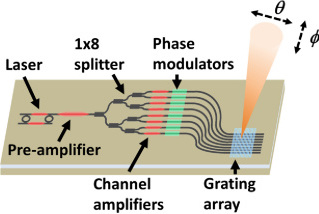
\includegraphics[width=12cm, height=8cm]{Figures/pic3}
%\caption{Circuit block digram }
%\label{blockGEN}
%\end{center}
%\end{figure}
%
%%
%\subsection{Phase Shifter}
%\label{phase shifters}
%The phase difference between the arrays will cause the beam scanning in direction of $\phi$
%Each waveguide well be doped with titled rectangles of p and n to create a PIN junction. The width of the depletion region and the carrier density in each waveguide is controlled by the applied reverse bias voltage to each waveguide. The tuning voltages are controlling the phase difference between the phased arrays which in return will control the scanning range in $\phi$ direction.
%
%\begin{equation}
%\beta_i \, = \, k_0 N_{eff}(n_i,p_i) \qquad i \; = \; 1 \, \dots \, N
%\end{equation}
%where $N $ is the number of phased arrays.
%\begin{equation}
%\Delta \phi \, = \, \beta L
%\end{equation}
%
%where $L$ is the length of the doped waveguide.
%
%\begin{center}
%\textbf{\LARGE To be Completed}
%\end{center}
%%
\subsection{Grating Couplers}
\label{gratingCouples}

Grating couples are being increasingly used in coupling out beams from the waveguides. In the GC structure, the wave propagates through the input waveguide, the periodic structure of the grating area will convert the wave to the leaky wave coupling off the surface of the waveguide to the air. In Telecom industry fiber optics are placed on top of the GC to couple light into it, but we in this research are using free space propagation for the LiDAR application.

The basic grating coupler is a periodic structure of teeth and groove with a grating period of $d$ and the coupling angle of $\theta.$ \cite{pub2000}

\subsubsection{Choose core material}
\label{core}
To analyze the physics of the GC, we start with the wave propagation in the waveguide with a propagation of $\beta_{s}$, because of the periodic structure there will be a leakage process from the waveguide which results in coupling out the light into the free space. This leakage process highly depends on the physical structure of the waveguides and grating such as index of reflection of the materials, the groove depth($t_g$), the pitch size($d$), length of grating ($L$) and the wavelength of the input light ($\lambda $). Because of the periodic structure of the GC, the leaky wave consist of an infinite space harmonic waves with a complex propagation of $k_n= \beta_n + i\alpha$ where $\alpha$ is the leakage factor and $\beta_n$ is the space harmonic propagation constant defined as below \cite{oe241821027beamwidth}, \cite{tamirPeng1977}:
\begin{equation}
\beta_n \, = \, \beta_0 \, + \, \frac{2n\pi}{d} \quad n=0 \, , \,  \pm1 \, , \, \pm2 \, , \, \dots
\end{equation}

Obviously the propagation is slower in the waveguide than in the free space for $\beta_s \, > \, k_0 $ where $k_0 \, =  \, \frac{2\pi}{\lambda}$.  Note that usually the leakage factor $\alpha$ is a very small value so $\beta_0 \, \simeq \, \beta_s$ and so we will have:
\begin{equation}
\beta_0 > k_0 (=2\pi / \lambda)
\end{equation}
On the other hand according to brag condition the radiation angle from the GC to the air is defined by
\begin{eqnarray}
\nonumber \sin(\theta_n)=\frac{\beta_n}{k_0} \quad n=0 \, , \,  \pm1 \, , \, \pm2 \, , \, \dots  \\
\sin(\theta_n)=\frac{\beta_0 +\frac{2n\pi}{d}}{k_0}\quad n=0 \, , \,  \pm1 \, , \, \pm2 \, , \, \dots  
\end{eqnarray}
Therefore in order to have a valid $\theta_n$ we should have $|\frac{\beta_0 +\frac{2n\pi}{d}}{k_0}| <1$. We also know that $\beta_0 > k_0$. This conclude that n must be negative.

Depending on the physical structure there will multiple outgoing beams, however in our application we wanted to have one strong outgoing beam so we design our GC for $n \, = \, -1$. For this purpose we must satisfy the following conditions:
\begin{eqnarray}
\nonumber |\beta_{-1}| \, < \, k0 \\
|\beta_{-2}| \, > \, k0
\label{betaTop}
\end{eqnarray}
Similar for the lower region (substrate) we should satisfy
\begin{equation}
|\beta_{-2}| \, > \, k0\sqrt{\epsilon_s}
\label{betaLow}
\end{equation}

Note that since $\epsilon_s > 1$ then  $|\beta_{-1}| \, < \, k0\sqrt{\epsilon_s}$ is automatically fulfilled.
Effective index of reflection (for thin film) is defined as 
\begin{equation}
N_{eff} \, = \, \beta_s/k_0 \, = \, \beta_0/k_0
\end{equation}
Rewriting equations (\ref{betaTop}) - (\ref{betaLow}) we will have
\begin{eqnarray*}
|\beta_0 -\frac{2\pi}{d}| <k_0 & => & |N_{eff}-\frac{\lambda}{d}| < 1\\
|\beta_0 -2\frac{2\pi}{d}| >k_0 & => & |N_{eff}-2\frac{\lambda}{d}| > 1\\ \\
|\beta_0 -2\frac{2\pi}{d}| >k_0 \sqrt{\epsilon_s} & => & |N_{eff}-\frac{\lambda}{d}| > \sqrt{\epsilon_s} \\
\end{eqnarray*}

or
\begin{eqnarray}
N_{eff}-\frac{\lambda}{d} < 1 \\
\frac{\lambda}{d} -N_{eff} > 1 \\
2\frac{\lambda}{d} - N_{eff} >1 \\
2\frac{\lambda}{d} - N_{eff} > \sqrt{\epsilon_s}
\end{eqnarray}
Also to avoid the Bragg condition we must have 
\begin{equation}
N_{eff} \, \neq \, \frac{\lambda}{d} 
\end{equation}

In Figure (\ref{neff1}) we showed the region for valid parameters to choose for forward or backward propagations
\begin{figure}[H]
\begin{center}
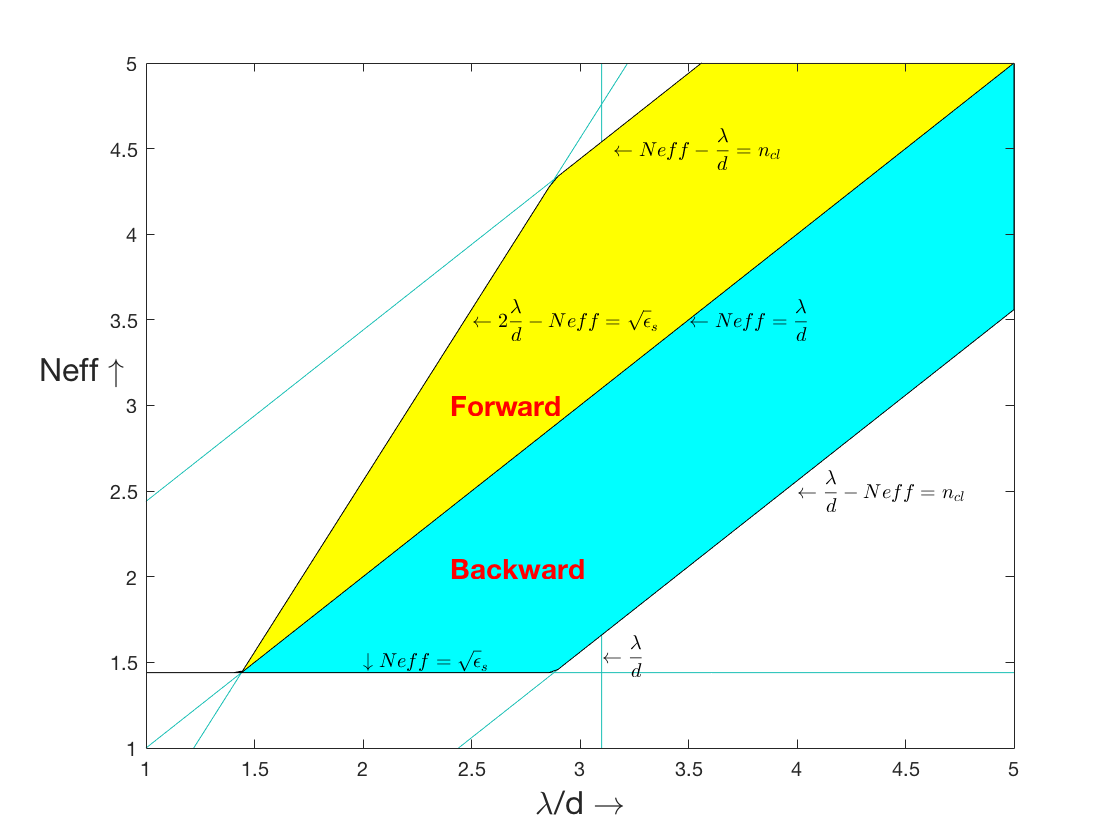
\includegraphics[width=12cm, height=8cm]{Figures/neffConstraint}
\caption{Valid Regions for forward or backward propagations}
\label{neff1}
\end{center}
\end{figure}

\subsubsection{Generate a Narrow beam (small FWHM)}
\label{smallFWHM}
To achieve a high resolution beam scanning, the outgoing beams must be very narrow. The FWHM of the beam  is highly depended to the group index of waveguide core ($N_{g_c}$) and the length of the grating $L$ as described in equation (\ref{lambdaFWHM}) \cite{hongChoSungFWHMsize} 
\begin{equation}
\delta \lambda_{FWHM} \, = \, \frac{\lambda^2}{2 \pi L N_{g_c}}
\label{lambdaFWHM}
\end{equation}
To get a narrow beam we need to increase the length and/or increase the group index. However for increasing the length, there are some limitation. Increasing the length will increase the transmission loss and also that will increase the size of the device. 
The other parameter to get us to a narrow beam is the group index, which is highly depended on the physical features of the grating such as the pitch size, duty cycle and etching depth. Among those the etching depth is process depended variable and there are limitation on it. Non uniform Shallow etching will have a huge impact on $N_{g_c}$ and $\delta \lambda_{FWHM} $,  however fabrication for non uniform shallow etching is costly and difficult, therefore we are replacing the effect of etching depth by using sub wavelength grating on the materials to achieve the desired small FWHM. 

\subsubsection{Effect of duty cycle}
\label{effectdutycycle}
\begin{equation}
N_{g} = f n_g \, + \, (1-f)n_t
\end{equation}

where $n_g$, $n_t$ and $N_{g}$ are index values for groove and teeth of GC and the grating area and $f$ is the duty cycle.

%\begin{center}
%\textbf{\LARGE To be Completed}
%\end{center}

\subsubsection{Design for minimum leakage}
\label{minleakage}

The duty cycle of the grating and the difference in permittivity of the grating and top cladding effects the leakage factor of the grating. For a rectangular grating this dependency in described as below:
\begin{equation}
\alpha \simeq (\epsilon_r \,- \, \epsilon_{cl})^2 \, \sin^2(\pi f /d)
\end{equation}

Where $\epsilon_r$ and $\epsilon_{cl}$ are the permittivity of the teeth and top cladding.

So to keep the leakage at minimum, we need to choose the teeth and top cladding from materials with not too far permittivity values. Here again we can take advance of our SWG design of the materials. We are going to use Silicon photonics platform and we don't have many options for our material selection, but using SWG we can engineer the materials with desired properties.

About the duty cycle we see that the leakage is at it's maximum value at $f \, = \,0.5$. So we need to design the duty cycle to be aways from 0.5. 

\subsubsection{Design for thickness of layers}
\label{thicknessLayers}
The propagation in different region of the structure is given by 
\begin{equation}
\gamma_{q_{-1}} \, = \, k_0\sqrt{\epsilon_q \, - \, (N \, - \frac{\lambda}{d})^2 }
\end{equation}
where $q$ identifies the layers (substrate, thin film, grating, cladding). Following the analysis in \cite{00248941} we know that for small values of $t_g$ ($t_{g}$ is the etch depth) where $|\gamma_{q_{-1}} t_g| <<1$ then $\alpha d \, \propto \, (t_g/d)^2$ meaning the decay is small but highly dependent on etch depth ($t_g$).\\
By increasing $t_g$ at some point the decay will be only of small oscillations with change of $t_g$ with a period of $\Lambda_{gn}$ given by
\begin{equation}
\Lambda_{g_{-1}} = \frac{2\pi}{\gamma_{g_{-1}} } =  \frac{\lambda}{\sqrt{\epsilon_g \, - \, (N \, - \frac{\lambda}{d})^2}  } 
\end{equation}

For this crossover point we have $t_{g_{cross}} \, = \, \frac{\Lambda_{g_{-1}}}{4} $. So for $t_g \, < t_{g_{cross}} $ the decay is small but highly dependent on the thickness, on the other hand for  $t_g \, > t_{g_{cross}} $ decay only have small variations with changing the thickness.

\subsubsection{pic2}
\label{pic2}
The outgoing beam has a FWHM divergence $\delta  \psi$ with a $\psi_s$ steering range, the resolution is $\psi_s / \delta  \psi$. Based on \cite{pic2} "To date, OPA steering resolution has been limited. To our knowledge, the widest demonstrated steering range of any OPA
was $51^{\circ}$; however, the beam divergence was relatively large $(3.3^{\circ})[9]$. The narrowest beam divergence was $0.3^{\circ}$; however, the steerable range was relatively small $(0.9^{\circ}) [12]$. The highest-resolution device had a resolution of 23, achieving the best ratio of steering range to beam divergence $(23^{\circ}$ and $1^{\circ}$, respectively) [10]."
The highest resolution in 2D using nonuniform etching and 32 emitters is about 23.


We using a simple and fabrication friendly method achieved resolution of 34 by sr


I wrote a MATLAB code where I define my constraints and parameters based on the above analysis and the code will define the physical features of the structure.







%
%%\lipsum[4] See Section \ref{sec:headings}.
%%
%%\subsection{Headings: second level}
%%\lipsum[5]
%%\begin{equation}
%%\xi _{ij}(t)=P(x_{t}=i,x_{t+1}=j|y,v,w;\theta)= {\frac {\alpha _{i}(t)a^{w_t}_{ij}\beta _{j}(t+1)b^{v_{t+1}}_{j}(y_{t+1})}{\sum _{i=1}^{N} \sum _{j=1}^{N} \alpha _{i}(t)a^{w_t}_{ij}\beta _{j}(t+1)b^{v_{t+1}}_{j}(y_{t+1})}}
%%\end{equation}
%%
%%\subsubsection{Headings: third level}
%%\lipsum[6]
%%
%%\paragraph{Paragraph}
%%\lipsum[7]
%\newpage
%\section{Examples of citations, figures, tables, references}
%\label{sec:others}
%\lipsum[8] \cite{kour2014real,kour2014fast} and see \cite{hadash2018estimate}.
%
%The documentation for \verb+natbib+ may be found at
%\begin{center}
%  \url{http://mirrors.ctan.org/macros/latex/contrib/natbib/natnotes.pdf}
%\end{center}
%Of note is the command \verb+\citet+, which produces citations
%appropriate for use in inline text.  For example,
%\begin{verbatim}
%   \citet{hasselmo} investigated\dots
%\end{verbatim}
%produces
%\begin{quote}
%  Hasselmo, et al.\ (1995) investigated\dots
%\end{quote}
%
%\begin{center}
%  \url{https://www.ctan.org/pkg/booktabs}
%\end{center}
%
%
%\subsection{Figures}
%\lipsum[10] 
%See Figure \ref{fig:fig1}. Here is how you add footnotes. \footnote{Sample of the first footnote.}
%\lipsum[11] 
%
%\begin{figure}
%  \centering
%  \fbox{\rule[-.5cm]{4cm}{4cm} \rule[-.5cm]{4cm}{0cm}}
%  \caption{Sample figure caption.}
%  \label{fig:fig1}
%\end{figure}
%
%\subsection{Tables}
%\lipsum[12]
%See awesome Table~\ref{tab:table}.
%
%\begin{table}
% \caption{Sample table title}
%  \centering
%  \begin{tabular}{lll}
%    \toprule
%    \multicolumn{2}{c}{Part}                   \\
%    \cmidrule(r){1-2}
%    Name     & Description     & Size ($\mu$m) \\
%    \midrule
%    Dendrite & Input terminal  & $\sim$100     \\
%    Axon     & Output terminal & $\sim$10      \\
%    Soma     & Cell body       & up to $10^6$  \\
%    \bottomrule
%  \end{tabular}
%  \label{tab:table}
%\end{table}
%
%\subsection{Lists}
%\begin{itemize}
%\item Lorem ipsum dolor sit amet
%\item consectetur adipiscing elit. 
%\item Aliquam dignissim blandit est, in dictum tortor gravida eget. In ac rutrum magna.
%\end{itemize}
%

\bibliographystyle{unsrt}  
\bibliography{references}  %%% Remove comment to use the external .bib file (using bibtex).
%%% and comment out the ``thebibliography'' section.


%%%% Comment out this section when you \bibliography{references} is enabled.
%\begin{thebibliography}{1}
%
%\bibitem{kour2014real}
%George Kour and Raid Saabne.
%\newblock Real-time segmentation of on-line handwritten arabic script.
%\newblock In {\em Frontiers in Handwriting Recognition (ICFHR), 2014 14th
%  International Conference on}, pages 417--422. IEEE, 2014.
%
%\bibitem{kour2014fast}
%George Kour and Raid Saabne.
%\newblock Fast classification of handwritten on-line arabic characters.
%\newblock In {\em Soft Computing and Pattern Recognition (SoCPaR), 2014 6th
%  International Conference of}, pages 312--318. IEEE, 2014.
%
%\bibitem{hadash2018estimate}
%Guy Hadash, Einat Kermany, Boaz Carmeli, Ofer Lavi, George Kour, and Alon
%  Jacovi.
%\newblock Estimate and replace: A novel approach to integrating deep neural
%  networks with existing applications.
%\newblock {\em arXiv preprint arXiv:1804.09028}, 2018.
%
%\end{thebibliography}


\end{document}
